\chapter{Implementation}

This chapter discusses how the software has been implemented. Section \ref{sec:implementation:overview} gives an overview about the tools and techniques being used. Sections \ref{sec:implementation:annotations}-\ref{sec:implementation:timecomplexityanalyser} will discuss the implementation of each existing module that has been introduced in the previous chapter.

\section{Overview}
\label{sec:implementation:overview}

\subsection{Important considerations}
As mentioned in previous chapters, one of the most important aspects of the product is to limit the observer effect. It is extremely important that the act of instrumenting and analysing the algorithm under test has the smallest possible impact on the algorithm's performance. Performance in programs that run on the JVM is also impacted be the garbage collection, given that when that happens all the threads are temporarily paused. This means that the act of collecting measurements must not have a big impact on memory, or the garbage collection will happen too often having a great impact on the algorithm's performance.

\noindent Considering this, it would be very hard, if not impossible, to come up with the theory supporting the instrumentation and measuring logic. Instead, different implementations will be attempted, discussed and compared in the following sections. All the different approaches will of course keep performance and memory usage in mind.

\subsection{Modules and dependencies}
The modules discussed in the previous chapters are defined as Maven\footnote{\url{https://maven.apache.org/}} modules. Maven is a tool that can be used to build and manage Java-based projects. Modules can be defined via a \code{pom.xml} file in the module's root folder, specifying the module group ID, artifact ID, version and the dependencies it has on other Maven modules. Maven dependencies could be defined by the user or could be 3rd party modules that exist in Maven public repositories. An example of a \code{pom.xml} file can be find in Appendix \ref{sec:appendices:examplepomfile}.

\subsection{Testing}
The concept of test-driven development (TDD) is applied to all modules. Tests that describe requirements are written prior to the implementation, then the implementation is added ensuring that the tests pass. This process inspires confidence, makes the software more robust and allows for easy refactoring. On top of that, benchmarks are used across modules that are performance-critical, ensuring the CPU time they use is minimal.

\subsection{Logging and debugging}
For this product's implementation, logging is very useful for:
\begin{itemize}
  \item Show debugging information, used to address problems such as bugs and performance issues
  \item Pointing to the line of code that caused an exception
  \item Better understanding of the application flow, especially for the users that don't know about the underlying software implementation
\end{itemize}

\noindent Simple Logging Facade for Java (SLF4J)\footnote{\url{https://www.slf4j.org/}} is an abstraction over different Java logging frameworks such as \code{java.util.logging}, \code{logback} and \code{log4j}. All the modules described in the following sections use the SLF4J API for logging.

\noindent The actual SLF4J implementation is only defined and configured at runtime, specifically in the root module (Time complexity analyser) via a Maven dependency and a configuration file. Logback is highly customisable and the log granularity can be configured on a per-package basis. During development it's often useful to show debugging information for the specific modules that are being worked on. Logging has an impact on performance so in the final implementation the logging should be minimal. Logback makes it very easy to change configuration via a \code{logback.xml} file that lives in the \code{src/main/resources} folder.

\noindent Most 3rd party Maven modules already use the SLF4J API but for the ones that don't SLF4J also offers bridges which redirect calls the legacy loggers to behave as if they were made to the SLF4J API instead.

\subsection{Disclaimer}
Code snippets included in the following sections have some differences compared to real product code:
\begin{itemize}
  \item Indentation in this document is 1 space character, compared to 2 spaces in the real code
  \item Log lines are sometimes removed
  \item Imports are omitted
  \item Some keywords, such as \code{final}, are sometimes removed
  \item \code{try-catch} blocks are sometimes omitted
\end{itemize}

\noindent All these differences are purely made for a question of space and to only show the part of the code that is relevant and important.

\section{Annotations}
\label{sec:implementation:annotations} 
This module defines a package \code{tech.dario.timecomplexityanalysis.annotations} which simply contains one single annotation, shown in Listing \ref{lis:measured}.

\noindent\begin{minipage}[c]{\linewidth}
\begin{lstlisting}[caption={Measured annotation},label=lis:measured]
public %%@interface%% Measured {
}
\end{lstlisting}
\end{minipage}

\noindent The annotation can be added to any method and any class and informs the agent that the entity should be time-measured (see next chapter).


\section{Agent}
\label{sec:implementation:agent} 
This module defines a package \code{tech.dario.timecomplexityanalysis.agent} containing the logic to instrument methods in order to measure how long they took and report it to the time recorder implementation. When built, this module produces a JAR file that can be used as a Java agent, as explained in Section \ref{sec:design:agent}.

\noindent The \code{MeasuringAgent} class in Listing \ref{lis:measuringagent} defines a \code{premain} method which is called after the Java Virtual Machine (JVM) is initialized and before the \code{main} method is called. This method registers a \code{MeasuringClassFileTransformer} which instruments classes as they get loaded. If the path to a configuration file is passed to the agent as an argument, the file is parsed and the configuration parameters are passed to the class file transformer. Otherwise it uses the default configuration (see Section \ref{sec:implementation:agent:configuration}).

\noindent\begin{minipage}[c]{\linewidth}
\begin{lstlisting}[breaklines,caption={$MeasuringAgent$ class},label=lis:measuringagent]
class MeasuringAgent {
 public static void premain(
   String agentArguments,
   Instrumentation instrumentation) {
  try {
   Config config = getConfigFromArguments(agentArguments);
   instrumentation.addTransformer(
     new MeasuringClassFileTransformer(config)
   );
  } catch (Exception e) {
   e.printStackTrace();
   System.exit(1);
  }
 }

 private static Config getConfigFromArguments(String agentArguments) throws IOException {
  if (agentArguments == null || agentArguments.trim().isEmpty()) {
   // No arguments
   return Config.getDefault();
  }

  return Config.fromJsonFilePath(agentArguments);
 }
}
\end{lstlisting}
\end{minipage}

\subsection{Configuration}
\label{sec:implementation:agent:configuration}
The agent can be configured with four different parameters:
\begin{enumerate}
  \item \textbf{\code{whitelist}}: a set of regexes\footnote{Regular expressions} indicating what methods to instrument. Default: empty set
  \item \textbf{\code{blacklist}}: a set of regexes indicating what methods to not instrument. Default: empty set
  \item \textbf{\code{excludeStandardJavaLibrary}}: a flag indicating whether to exclude classes that are part of the standard Java 8 library\footnote{\code{java}, \code{javax}, \code{jdk}, \code{sun}, \code{com.oracle.net}, \code{com.sun}, \code{org.ietf.jgss} and \code{org.jcp.xml.dsig.internal} packages}. Default: \code{true}
  \item \textbf{\code{excludeStandardScalaLibrary}}:  a flag indicating whether to exclude classes that are part of the standard Scala library\footnote{\code{scala} package}. Default: \code{true}
\end{enumerate}

\noindent Listing \ref{lis:config1} shows an example of configuration which instructs the agent to insturment any method in the \code{tech.dario.timecomplexityanalysis.testalgorithm} package, excluding any method starting with \code{get}. The regexes specified in the \code{whitelist} and \code{blacklist} parameters should be in a format accepted by the \code{compile} method of \code{java.util.regex.Pattern}\footnote{\url{https://docs.oracle.com/javase/8/docs/api/java/util/regex/Pattern.html}}. For example, method \code{tech.dario.timecomplexityanalysis.testalgorithm.MyClass.getName()} is both whitelisted and blacklisted. The whitelist regex matches \code{tech.dario.timecomplexityanalysis.testalgorithm} while the blacklist element matches \code{tech.dario.timecomplexityanalysis.testalgorithm.MyClass.get}. Because the blacklist element is more targeted, it takes priority over the whitelist element so the method is not instrumented (see Section \ref{sec:implementation:agent:transformation} for more details).

\noindent\begin{minipage}[c]{\linewidth}
\begin{lstlisting}[breaklines,caption={Configuration JSON file example},label=lis:config1,style=json]
{
 "whitelist": [
  "^tech\\.dario\\.timecomplexityanalysis\\.testalgorithm\\."
 ],
 "blacklist": [
  "^tech\\.dario\\.timecomplexityanalysis\\.testalgorithm\\..+\\.get"
 ],
 "excludeStandardJavaLibrary": true,
 "excludeStandardScalaLibrary": true
}
\end{lstlisting}
\end{minipage}

\subsection{Transformation}
\label{sec:implementation:agent:transformation}

\code{MeasuringClassFileTransformer} constructor in Listing \ref{lis:measuringclassfiletransformer:constructor} accepts an instance of \code{Config} and saves it in a local field which can be accessed in the transformation. It also compiles the whitelist and blacklist regexes converting them from \code{String} to \code{Pattern} and saves them in two local fields of type \code{Set<Pattern>} called \code{whitelistPatterns} and \code{blacklistPatterns} respectively. Doing this step upfront decreases the time the transformation takes as it ensures that each regex is only compiled once as opposed to compiling it each time a method is checked for instrumentation.

\noindent\begin{minipage}[c]{\linewidth}
\begin{lstlisting}[breaklines,caption={$MeasuringClassFileTransformer$ initialization},label=lis:measuringclassfiletransformer:constructor]
class MeasuringClassFileTransformer implements ClassFileTransformer {

 ...

 private final Config config;
 private final Set<Pattern> whitelistPatterns;
 private final Set<Pattern> blacklistPatterns;

 public MeasuringClassFileTransformer(Config config) {
  this.config = config;
  this.whitelistPatterns = stringSetToPatternSet(config.getWhitelist());
  this.blacklistPatterns = stringSetToPatternSet(config.getBlacklist());
 }

 ...

 private Set<Pattern> stringSetToPatternSet(Set<String> stringSet) {
  if (stringSet == null) {
   return null;
  }

  return stringSet
    .stream()
    .map(Pattern::compile)
    .collect(Collectors.toSet());
 }
}
\end{lstlisting}
\end{minipage}

\noindent \code{MeasuringClassFileTransformer} implements \code{interface} \code{java.lang.instrument.ClassFileTransformer}\footnote{\url{https://docs.oracle.com/javase/8/docs/api/java/lang/instrument/ClassFileTransformer.html}} which defines method \code{transform} shown in Listing \ref{lis:measuringclassfiletransformer:transform}. By implementing this interface, \code{MetricAgent} can use \code{MeasuringClassFileTransformer} as one of its transformers and because of that each class being loaded in the JVM will pass through this transformer for optional instrumentation. This class' responsibility is to determine whether the class being loaded should be instrumented and if so to instrument it.

\noindent\begin{minipage}[c]{\linewidth}
\begin{lstlisting}[breaklines,caption={$MeasuringClassFileTransformer.transform$ implementation},label=lis:measuringclassfiletransformer:transform]
$$@Override
public byte[] transform(
  ClassLoader loader,
  String fullyQualifiedClassName,
  Class<?> classBeingRedefined,
  ProtectionDomain protectionDomain,
  byte[] classfileBuffer) throws IllegalClassFormatException {
 if (isClassExcludedByName(fullyQualifiedClassName)) {
  return null;
 }

 String className = fullyQualifiedClassName.replace("/", ".");
 CtClass ctClass = ClassPool.getDefault().get(className);
 if (isClassExcludedByImplementation(ctClass)) {
  return null;
 }

 declareAndInstantiateTimeRecorder(ctClass);

 boolean isClassModified = instrumentMeasuredMethods(ctClass);
 if (!isClassModified) {
  return null;
 }

 return ctClass.toBytecode();
}
\end{lstlisting}
\end{minipage}


\noindent The transformer first uses private method \code{isClassExcludedByName} to check whether the class should be excluded from instrumentation based on its fully qualified class name. As the documentation states, the name of the class passed in the method is in the internal form of fully qualified class names as defined in \textit{The Java Virtual Machine Specification} (e.g. \code{java/util/List}). A class will be excluded based on its fully qualified name if:
\begin{itemize}
  \item It's part of the standard Java library and the \code{excludeStandardJavaLibrary} configuration parameter is set to true, or
  \item It's part of the standard Scala library and the \code{excludeStandardScalaLibrary} configuration parameter is set to true, or
  \item It's part of the \code{javaassist} package or the \code{tech.dario.timecomplexityanalysis.timerecorder} package (this is to avoid instrumenting classes that are needed for instrumentation itself)
\end{itemize}

\noindent If the class is excluded, the method returns \code{null} which instructs the JVM that this class should be loaded without any instrumentation applied. Otherwise it loads the class from the default \code{ClassPool}\footnote{\url{https://jboss-javassist.github.io/javassist/html/javassist/ClassPool.html}} and uses private method \code{isClassExcludedByImplementation} to check whether the class should be excluded based on its implementation. In the context of instrumentation the term \enquote{class} is used in a more generic way and includes annotations, arrays, enums, interfaces and primitives too. \code{MeasuringClassFileTransformer} excludes any class that is not an actual class (i.e. defined with the \code{class} keyword) from instrumentation by returning \code{null}.

\noindent Now the time recorder is declared and instantiated in the class by using the private method \code{declareAndInstantiateTimeRecorder}. It instruments the class by declaring a private, static and final field called \code{\_AGENT\_TIME\_RECORDER} as shown in Listing \ref{lis:measuringclassfiletransformer:agenttimerecorder}. Note that at this point the instrumented class is using the time recorder API to report time and is unaware of what the actual time recorder implementation is. Section \ref{sec:implementation:timerecorderapi} will explain how the time recorder implementation is injected into the instrumented classes.

\noindent\begin{minipage}[c]{\linewidth}
\begin{lstlisting}[breaklines,caption={$\_AGENT\_TIME\_RECORDER$ initialization},label=lis:measuringclassfiletransformer:agenttimerecorder]
private final static tech.dario.timecomplexityanalysis.timerecorder.api.TimeRecorder _AGENT_TIME_RECORDER = tech.dario.timecomplexityanalysis.timerecorder.api.StaticTimeRecorderFactory.getTimeRecorder();
\end{lstlisting}
\end{minipage}

\noindent The whitelisted methods now get instrumented using the private method \code{instrumentMeasuredMethods}. For each method of each class that is not excluded, the agent uses the logic in Listing \ref{lis:measuringclassfiletransformer:ismethodmeasured} to determine whether the method should be instrumented. It finds the best-matching whitelist regex and the best-matching blacklist regex. The longer the match, the better and more targeted it is considered to be. If the best-matching whitelist regex is more targeted than the best-matching blacklist regex (or as targeted, i.e. whitelists have priority over blacklists) then the method is instrumented, otherwise it is not. If no matching regexes are found for the method, the same logic is applied on the method's class name. \noindent If a method is annotated with \code{@Measured}, it is always instrumented with no exceptions (blacklist regexes are ignored in this case). If a class is annotated with \code{@Measured}, each of its methods is instrumented unless explicitly blacklisted.

\noindent\begin{minipage}[c]{\linewidth}
\begin{lstlisting}[breaklines,caption={$MeasuringClassFileTransformer.isMethodMeasured$ implementation},label=lis:measuringclassfiletransformer:ismethodmeasured]
private boolean isMethodMeasured(CtClass ctClass, CtMethod ctMethod) {
 if (ctMethod.hasAnnotation(Measured.class)) {
  return true;
 }

 InstrumentationStatus methodInstrumentationStatus = getInstrumentationStatus(ctMethod.getLongName());
 if (methodInstrumentationStatus == InstrumentationStatus.WHITELISTED) {
  return true;
 }

 if (methodInstrumentationStatus == InstrumentationStatus.BLACKLISTED) {
  return false;
 }

 if (methodInstrumentationStatus == InstrumentationStatus.INDIFFERENT) {
  if (ctClass.hasAnnotation(Measured.class)) {
   return true;
  }

  InstrumentationStatus classInstrumentationStatus = getInstrumentationStatus(ctClass.getName());
  if (classInstrumentationStatus == InstrumentationStatus.WHITELISTED) {
   return true;
  }

  if (classInstrumentationStatus == InstrumentationStatus.BLACKLISTED) {
   return false;
  }
 }
    
 return false;
}

private InstrumentationStatus getInstrumentationStatus(String entityName) {
 int bestWhitelistMatch = findBestMatchingPatternLength(entityName, whitelistPatterns);
 int bestBlacklistMatch = findBestMatchingPatternLength(entityName, blacklistPatterns);
 if (bestWhitelistMatch == 0 && bestBlacklistMatch == 0) {
  return InstrumentationStatus.INDIFFERENT;
 }

 if (bestBlacklistMatch > bestWhitelistMatch) {
  return InstrumentationStatus.BLACKLISTED;
 }

 return InstrumentationStatus.WHITELISTED;
}

private int findBestMatchingPatternLength(final String input, final Set<Pattern> patternsSet) {
 return patternsSet
   .stream().map(pattern -> pattern.matcher(input))
   .filter(Matcher::find).map(matcher -> matcher.group(0).length())
   .mapToInt(i -> i).max().orElse(0);
}
\end{lstlisting}
\end{minipage}

\noindent When a method is elected for instrumentation, its implementation is changed to record measurements. The first approach (see Listing \ref{lis:measuringclassfiletransformer:firstmethodinstrumentationexample}) involved measuring time taken in nanoseconds and the thread \code{StackTrace} to the time reporter just before the method returned.

\noindent\begin{minipage}[c]{\linewidth}
\begin{lstlisting}[breaklines,caption={Method instrumentation example (first approach)},label=lis:measuringclassfiletransformer:firstmethodinstrumentationexample]
$$@Measured
public void myMethod() {
 StackTraceElement[] _agent_stackTrace = Thread.currentThread().getStackTrace();
 long _agent_startTime = System.nanoTime();

 // Original implementation here

 _AGENT_TIME_RECORDER.reportTime(System.nanoTime() - _agent_startTime, _agent_stackTrace);
}
\end{lstlisting}
\end{minipage}

\noindent Benchmarks showed how this implementation always slowed down the instrumented method by a constant amount of time in the order of magnitude of \SI{10}{\micro\second} on a \SI{2.8}{\giga\hertz} machine. This is an enormous amount of time that would have a big impact on the observer effect, hence drastically compromising the time complexity calculation. Profiling the agent showed how the culprit is the call to get the stack trace.

\noindent The instrumentation logic has to be as light as possible to not have an impact on the measurement of the time complexity of the algorithm under test. The second approach (see Listing \ref{lis:measuringclassfiletransformer:secondmethodinstrumentationexample}) removes the slow call to get the stack trace and instead simply informs the time recorder of when the method has started and when it has finished, passing along the unique method long name (which consists of package name, class name, method name and arguments types). The time recorder will have more responsibilities and will be a bit more complicated because, on top of having to calculate the time taken it will also require to work out the stack trace of each time report. Delegating the complex logic to the time recorder is a much better approach as it can be done in a separate thread and/or after all the recording rounds have run, hence greatly reducing the observer effect.

\noindent\begin{minipage}[c]{\linewidth}
\begin{lstlisting}[breaklines,caption={Method instrumentation example (second approach)},label=lis:measuringclassfiletransformer:secondmethodinstrumentationexample]
$$@Measured
public void myMethod() {
 _AGENT_TIME_RECORDER.methodStarted("myPackage.myClass.myMethod()");

 // Original implementation here

 _AGENT_TIME_RECORDER.methodFinished("myPackage.myClass.myMethod()");
}
\end{lstlisting}
\end{minipage}


\noindent The private method \code{instrumentMeasuredMethods} mentioned above returns a boolean indicating whether any of the methods in the class have been instrumented. If no methods have been instrumented, the \code{transform} method returns \code{null} meaning that the original instrumentation done in private method \code{declareAndInstantiateTimeRecorder} is undone.

\subsection{Limitations}
\label{sec:implementation:agent:limitations}
Some classes are pre-loaded in the JVM, such as some of the classes that are part of the Java standard library. Because they're pre-loaded, these classes don't go though the transformer and for that reason are never instrumented. Java could retransform pre-loaded classes but the documentation\footnote{\url{https://docs.oracle.com/javase/8/docs/api/java/lang/instrument/Instrumentation.html}} states:

\enquote{The retransformation must not add, remove or rename fields or methods, change the signatures of methods, or change inheritance}

\noindent Because \code{MeasuringClassFileTransformer} adds a field \code{\_AGENT\_TIME\_RECORDER}, retrasformation is not allowed and as a consequence any pre-loaded classes cannot be analysed. The field is not strictly necessary as it could simply be instantiated and initialised inside the instrumented method instead. Doing so would imply slowing down each instrumented method as the initialisation takes CPU time.

\section{Time recorder API}
\label{sec:implementation:timerecorderapi}
The main responsibility of this module is to provide an abstraction over the actual time recording implementation. The main interface is shown in Listing \ref{lis:timerecorderapi:timerecorderinterface} and has 4 methods:
\begin{itemize}
  \item \textbf{\code{start}}: used when a new recording is starting, so that the internal data structures used by the implementation, if any, can be initialised
  \item \textbf{\code{methodStarted}}: used when a new instrumented method is starting doing its work. The subject instrumented method long name is passed to the implementation
  \item \textbf{\code{methodFinished}}: used when a new instrumented method is finished doing its work. The subject instrumented method long name is passed to the implementation
  \item \textbf{\code{stop}}: used when the current recording is finished (i.e. no more instrumented methods will start or stop from this point on). The implementation can then transform its internal data structures and return the recorded data as an instance of \code{MergeableTree<Measurement>} (see next sections)
\end{itemize}

\noindent\begin{minipage}[c]{\linewidth}
\begin{lstlisting}[breaklines,caption={TimeRecorder interface},label=lis:timerecorderapi:timerecorderinterface]
public interface TimeRecorder {
 void start() throws Exception;

 void methodStarted(String methodLongName);
 void methodFinished(String methodLongName);

 MergeableTree<Measurement> stop() throws Exception;
}
\end{lstlisting}
\end{minipage}

\noindent As mentioned before, the time recorder implementation to use will be decided by the root module (Time complexity analyser). This means that  the algorithm under test, whose methods are instrumented, must not be tied to the time recorder implementation, but must rely on the API instead. The challenge that arises is then how to ensure that the instrumented methods have access to the time recorder implementation, in order to call its \code{methodStarted} and \code{methodFinished} methods. Usually, when an object needs to use another object in order to do its job, the former takes the latter as a constructor argument. An entity responsible for running the program will then ensure that all the long-lived objects (often called services) are created and passed correctly to the constructors of all the services. This pattern is known as dependency injection \footnote{\url{https://martinfowler.com/articles/injection.html}}. Unfortunately, this pattern cannot be applied in this circumstance, as none of the modules have control over how the objects inside the algorithm under test are instantiated.

\noindent A good alternative is to retrieve the implementation via the call to a public static method defined in the API, as previously seen in Listing \ref{lis:measuringclassfiletransformer:agenttimerecorder}. Again, the problem is that the API does not know about the implementation, but there is a small trick that allows this approach to work. The class \code{StaticTimeRecorderFactory} has a static method \code{getTimeRecorder()} to get the time recorder implementation. It is inspired by SLF4J \code{LoggerFactory}, which has a static method \code{getLogger(...)} to get the logger implementation\footnote{\url{https://github.com/qos-ch/slf4j/blob/master/slf4j-api/src/main/java/org/slf4j/LoggerFactory.java}}. When \code{StaticTimeRecorderFactory.getTimeRecorder()} is called, it uses \code{StaticTimeRecorderBinder} to get the time recorder implementation. The API contains a dummy implementation of \code{StaticTimeRecorderBinder} (see Listing \ref{lis:timerecorderapi:statictimerecorderbinderdummy}), but the idea is to swap this with the real implementation when the implementation is added as a Maven dependency. In fact this class is only used so that the whole module can be compiled, but the associated compiled \code{.class} file is removed just before packaging it inside the Maven artifact.

\noindent\begin{minipage}[c]{\linewidth}
\begin{lstlisting}[breaklines,caption={StaticTimeRecorderBinder dummy implementation},label=lis:timerecorderapi:statictimerecorderbinderdummy]
package tech.dario.timecomplexityanalysis.timerecorder.impl;

class StaticTimeRecorderBinder {
 private static final StaticTimeRecorderBinder SINGLETON = new StaticTimeRecorderBinder();

 public static final StaticTimeRecorderBinder getSingleton() {
  return SINGLETON;
 }

 private StaticTimeRecorderBinder() {
  throw new UnsupportedOperationException("This code should have never made it into time-recorder-api");
 }

 public TimeRecorder getTimeRecorder() {
  throw new UnsupportedOperationException("This code should never made it into time-recorder-api");
 }

 public String getTimeRecorderFactoryClassStr() {
  throw new UnsupportedOperationException("This code should never made it into time-recorder-api");
 }
}
\end{lstlisting}
\end{minipage}

\noindent In order for this trick to work, the time recorder implementation will have to define the class so that its fully qualified name is \code{tech/dario/timecomplexityanalysis/timerecorder/impl/StaticTimeRecorderBinder}. The class will need to define the same 3 public methods:

\begin{itemize}
  \item \textbf{\code{static} \code{StaticTimeRecorderBinder} \code{getSingleton()}}: used by \code{StaticTimeRecorderFactory} to get a singleton instance of the \code{StaticTimeRecorderBinder}
  \item \textbf{\code{TimeRecorder} \code{getTimeRecorder()}}: used to get the time recorder
  \item \textbf{\code{String} \code{getTimeRecorderClassStr()}} used to return the implementation name (purely used to distinguish it from other implementations)
\end{itemize}

\subsection{Data structures}
\label{sec:implementation:timerecorderapi:datastructures}

The API also offers some powerful data structures in order for other modules to be able to easily manage and transform the recorded data. Figure \ref{fig:timerecorerapi:datastructuresclassdiagram} shows a class diagram of all the different data structures that exist within this module. Note that this class diagram only shows inheritances and implementations and does not include associations, compositions and aggregations. It also omits information about the classes type parameters.

\begin{figure}
  \centering
  \begin{tikzpicture}[rotate=90, transform shape]
    \umlsimpleclass[y=0.0em, x=0.0em, width=9.0em, type=abstract]{AbstractNode}
    \umlsimpleinterface[y=0.0em, x=14.0em, width=9.0em]{Mergeable}
    \umlsimpleclass[y=0.0em, x=28.0em, width=9.0em, type=abstract]{AbstractTree}
    \umlsimpleclass[y=-12.0em, x=9.0em, width=9.0em]{MergeableCollection}
    \umlsimpleclass[y=-12.0em, x=19.0em, width=9.0em]{Measurement}
    \umlsimpleclass[y=-6.0em, x=-5.0em, width=9.0em]{SimpleNode}
    \umlsimpleclass[y=-6.0em, x=5.0em, width=9.0em]{MergeableNode}
    \umlsimpleclass[y=-6.0em, x=23.0em, width=9.0em]{MergeableTree}
    \umlsimpleclass[y=-6.0em, x=33.0em, width=9.0em]{SimpleTree}
        
    \umlinherit[geometry=|-|]{SimpleNode}{AbstractNode}
    \umlinherit[geometry=|-|]{MergeableNode}{AbstractNode}
    \umlimpl[geometry=|-|, anchor1=32]{MergeableNode}{Mergeable}
        
    \umlimpl[geometry=|-|, weight=0.3]{MergeableCollection}{Mergeable}
    \umlimpl[geometry=|-|, weight=0.3]{Measurement}{Mergeable}
        
    \umlimpl[geometry=|-|, anchor1=147]{MergeableTree}{Mergeable}
    \umlinherit[geometry=|-|]{MergeableTree}{AbstractTree}
    \umlinherit[geometry=|-|]{SimpleTree}{AbstractTree}
  \end{tikzpicture}
  \caption{Data structures class diagram}
  \label{fig:timerecorerapi:datastructuresclassdiagram}
\end{figure}

\subsubsection{AbstractNode}
\code{AbstractNode} is an abstract generic class defined as shown in Listing \ref{lis:timerecorderapi:abstractnodeclassdefinition}.

\noindent\begin{minipage}[c]{\linewidth}
\begin{lstlisting}[breaklines,caption={AbstractNode class definition},label=lis:timerecorderapi:abstractnodeclassdefinition]
public abstract class AbstractNode<T, S extends AbstractNode<T, S>> {
 private final String name;
 private S parent;
 private T data;
 private Map<String, S> children;

 // ...
}
\end{lstlisting}
\end{minipage}

\noindent It has 2 type paramenters: \code{T} is the type of the data the node contains while \code{S} is the reference to the node type itself. The latter is useful mainly to make the definition a bit more clear and understandable.

\noindent It has a \code{name} field to uniquely identify it, a \code{parent} field to store the reference to its parent, a \code{data} field to store the data and a \code{children} field containing a reference to all the children. Children are stored in a \code{Map<String, S>} (where \code{S} is the type of the node), so that children can be looked up by name in constant time.

\noindent Besides basic methods such as \code{add(...)} and getters, this class has a powerful \code{map} method (shown in Listing \ref{lis:timerecorderapi:abstractnodemapmethoddefinition}) to return a copy of the node with a function applied to the node and each of its children, recursively.

\noindent\begin{minipage}[c]{\linewidth}
\begin{lstlisting}[breaklines,caption={AbstractNode map method definition},label=lis:timerecorderapi:abstractnodemapmethoddefinition]
public <T2, S2 extends AbstractNode<T2, S2>> S2 map(Function<? super S, ? extends S2> mapper) {
 Queue<NodesPair<T, S, T2, S2>> queue = new LinkedList<>();

 S2 newRootNode = mapper.apply((S)this);

 queue.add(new NodesPair<>((S)this, newRootNode));

 while (!queue.isEmpty()) {
  NodesPair<T, S, T2, S2> nodes = queue.remove();

  S node = nodes.getNode1();
  S2 newNode = nodes.getNode2();

  for (S childNode : node.getChildren().values()) {
   S2 newChildNode = mapper.apply(childNode);
   newNode.add(newChildNode);
   queue.add(new NodesPair<>(childNode, newChildNode));
  }
 }

 return newRootNode;
}
\end{lstlisting}
\end{minipage}

\noindent The method uses a non-recursive implementation of Breadth-first search (BFS) \cite{EFM59} to traverse the tree. To start, the node and its transformed version (after applying the mapping function) are added to the BFS queue in an instance of \code{NodesPair}, a simple object that stores two nodes in memory (\code{node1} is the original one, \code{node2} is the transformed one). Then, every time an element is popped from the queue, a loop goes through all the \code{node1} children, applying the mapping function to each one of them. The transformed children are added to the \code{node2} that the BFS loop is currently visiting, and are also added to the BFS queue, again in instances of \code{NodesPair} together with their original counterparts.

\subsubsection{Mergeable}
\code{Mergeable} is an interface defined as shown in Listing \ref{lis:timerecorderapi:mergeableinterfacedefinition}.

\noindent\begin{minipage}[c]{\linewidth}
\begin{lstlisting}[breaklines,caption={Mergeable interface definition},label=lis:timerecorderapi:mergeableinterfacedefinition]
public interface Mergeable<T extends Mergeable<T>> {
 T mergeWith(T mergeable);
}
\end{lstlisting}
\end{minipage}

\noindent It has a type parameter \code{T} that refers to its own type. It defines a \code{mergeWith(...)} that is needed to indicate that the classes implementing this interface are mergeable. When a class is mergeable, it needs to define a \code{mergeWith(...)} method, which takes another object of the same type, merges it with itself and returns the merged object. Useful usages of this interface will be presented in the following sections.

\subsubsection{AbstractTree}

\code{AbstractTree} is an abstract class defined as shown in Listing \ref{lis:timerecorderapi:abstracttreeclassdefinition}.

\noindent\begin{minipage}[c]{\linewidth}
\begin{lstlisting}[breaklines,caption={AbstractTree class definition},label=lis:timerecorderapi:abstracttreeclassdefinition]
public abstract class AbstractTree<T, S extends AbstractNode<T, S>, R extends AbstractTree<T, S, R>> {
 protected S rootNode;
 
 // ...
}
\end{lstlisting}
\end{minipage}

\noindent It has 3 type paramenters: \code{T} is the type of the data the tree contains, \code{S} is the type of node the tree uses and \code{R} is the reference to the tree type itself. As per \code{AbstractNode}, both \code{S} and \code{R} are useful mainly to make the definition a bit more clear and understandable.

\noindent It has a single field \code{rootNode}, which stores the reference to the tree's root node.

\noindent Besides basic methods to add nodes and to get the root node, this class also has a powerful \code{map} method (shown in Listing \ref{lis:timerecorderapi:abstracttreemapmethoddefinition}) to return a copy of the tree with a function applied to each of its nodes.

\noindent\begin{minipage}[c]{\linewidth}
\begin{lstlisting}[breaklines,caption={AbstractTree map method definition},label=lis:timerecorderapi:abstracttreemapmethoddefinition]
public <T2, S2 extends AbstractNode<T2, S2>, R2 extends AbstractTree<T2, S2, R2>> R2 map(Function<? super S2, ? extends R2> treeCreator, Function<? super S, ? extends S2> nodeMapper) {
 S2 newRootNote = rootNode.map(nodeMapper);
 return treeCreator.apply(newRootNote);
}
\end{lstlisting}
\end{minipage}

\noindent In this case the method takes two functions: \code{treeCreator} and \code{nodeMapper}. \code{treeCreator} takes the new root node as input and returns a new tree using that node as the root node. \code{nodeMapper} is the node transformer and is simply applied to the tree's root node via a call to its \code{map(...)} method shown before in Listing \ref{lis:timerecorderapi:abstractnodemapmethoddefinition}. The combination of the two returns a new tree with each of its node mapped using the supplied mapping function.

\subsubsection{SimpleNode}

\code{SimpleNode} is a concrete class defined as shown in Listing \ref{lis:timerecorderapi:simplenodeclassdefinition}.

\noindent\begin{minipage}[c]{\linewidth}
\begin{lstlisting}[breaklines,caption={SimpleNode class definition},label=lis:timerecorderapi:simplenodeclassdefinition]
class SimpleNode<T> extends AbstractNode<T, SimpleNode<T>> {
 public SimpleNode(final String name) {
  this(name, null);
 }

 public SimpleNode(final String name, final T data) {
  super(name, data);
 }
}
\end{lstlisting}
\end{minipage}

\noindent As the name suggests, it's the simplest possible implementation of \code{AbstractNode}. It represent a simple node that stores data of type \code{T}.

\subsubsection{MergeableNode}

\code{MergeableNode} is a concrete class defined as shown in Listing \ref{lis:timerecorderapi:mergeablenodeclassdefinition}.

\noindent\begin{minipage}[c]{\linewidth}
\begin{lstlisting}[breaklines,caption={MergeableNode class definition},label=lis:timerecorderapi:mergeablenodeclassdefinition]
class MergeableNode<T extends Mergeable<T>> extends AbstractNode<T, MergeableNode<T>> implements Mergeable<MergeableNode<T>> {
 public MergeableNode(String name) {
  this(name, null);
 }

 public MergeableNode(String name, T data) {
  super(name, data);
 }

 public void addData(T data) {
  mergeData(data);
 }
  
 // ...

 private void mergeData(T otherData) {
  if (!this.hasData()) {
    setData(otherData);
  } else if (otherData != null) {
    setData(getData().mergeWith(otherData));
  }
 }
\end{lstlisting}
\end{minipage}

\noindent This class represents a node that can be merged with another node of the same type. It has a type parameter \code{T}, where \code{T} has to be a class that implements \code{Mergeable}. On top of all methods offered by \code{AbstractNode}, which this class extends, it allows adding data to the node. If the node already has data, it is merged with the new value, otherwise the new value is just set as the node data.

\noindent Because this class itself implements the \code{Mergeable} interface, it needs to implement a \code{mergeWith(...)} method, shown in Listing \ref{lis:timerecorderapi:mergeablenodemergewithmethoddefinition}.

\noindent\begin{minipage}[c]{\linewidth}
\begin{lstlisting}[breaklines,caption={MergeableNode mergeWith method definition},label=lis:timerecorderapi:mergeablenodemergewithmethoddefinition]
$$@Override
public MergeableNode<T> mergeWith(MergeableNode<T> otherNode) {
 if (otherNode == null) {
  return this;
 }

 if (!getName().equals(otherNode.getName())) {
  String message = String.format("Cannot merge MergeableNode '%s' with MergeableNode '%s' as names are different", getName(), otherNode.getName());
  throw new RuntimeException(message);
 }

 MergeableNode<T> mergedNode = new MergeableNode<>(getName(), getData());

 // Merge node data
 mergedNode.mergeData(otherNode.getData());

 // Add all children that are in this node, merging them with the ones in the other node when they exist
 for (Map.Entry<String, MergeableNode<T>> child : getChildren().entrySet()) {
  String childName = child.getKey();
  if (otherNode.hasChild(childName)) {
   mergedNode.add(child.getValue().mergeWith(otherNode.getChild(childName)));
  } else {
   mergedNode.add(child.getValue());
  }
 }

 // Add all children that are in otherNode but not in this node
 for (Map.Entry<String, MergeableNode<T>> child : otherNode.getChildren().entrySet()) {
  String childName = child.getKey();
  if (!mergedNode.hasChild(childName)) {
   mergedNode.add(child.getValue());
  }
 }

 return mergedNode;
}
\end{lstlisting}
\end{minipage}

\noindent First, the subject node's data is merged with the other node's data. Then, for each child in the subject node, the correspondent child (i.e. with the same name) is looked up in the other node and if found they are merged using the \code{mergeWith(...)} method. If not found, the subject node's data is used instead. Because there could be some children in the other node that are not present in the subject node, it is necessary to loop through all the children in the other node that are not present in the current node and add them to the merged node. Note that because there is a recursive call to the \code{mergeWith(...)} method, the whole node hierarchy will be merged.

\subsubsection{MergeableTree}

\code{MergeableTree} is a concrete class defined as shown in Listing \ref{lis:timerecorderapi:mergeabletreeclassdefinition}.

\noindent\begin{minipage}[c]{\linewidth}
\begin{lstlisting}[breaklines,caption={MergeableTree class definition},label=lis:timerecorderapi:mergeabletreeclassdefinition]
class MergeableTree<T extends Mergeable<T>> extends AbstractTree<T, MergeableNode<T>, MergeableTree<T>> implements Mergeable<MergeableTree<T>> {
 public MergeableTree() {
  this(new MergeableNode<>("root", null));
 }

 public MergeableTree(MergeableNode<T> rootNode) {
  super(rootNode);
 }

 $$@Override
 public MergeableTree<T> mergeWith(MergeableTree<T> otherTree) {
  MergeableNode<T> otherRootNode = null;
  if (otherTree != null) {
   otherRootNode = otherTree.getRootNode();
  }
  return new MergeableTree<>(getRootNode().mergeWith(otherRootNode));
 }
}
\end{lstlisting}
\end{minipage}

\noindent This class represents a tree that can be merged with another tree of the same type. It has a type parameter \code{T}, where \code{T} has to be a class that implements \code{Mergeable}. It extends \code{AbstractTree} and, given it also implements the \code{Mergeable} interface, on top of all methods offered by \code{AbstractTree} it needs to implement a \code{mergeWith(...)} method. The \code{mergeWith(...)} method simply merges the root node of the subject tree with the root node of the other tree and then returns a new instance of \code{MergeableTree}, with the merged node as the root node.

\subsubsection{SimpleTree}

\code{SimpleTree} is a concrete class defined as shown in Listing \ref{lis:timerecorderapi:simpletreeclassdefinition}.

\noindent\begin{minipage}[c]{\linewidth}
\begin{lstlisting}[breaklines,caption={SimpleTree class definition},label=lis:timerecorderapi:simpletreeclassdefinition]
class SimpleTree<T> extends AbstractTree<T, SimpleNode<T>, SimpleTree<T>> {
 public SimpleTree() {
  this(new SimpleNode<>("root", null));
 }

 public SimpleTree(SimpleNode<T> rootNode) {
  super(rootNode);
 }
}
\end{lstlisting}
\end{minipage}

\noindent As the name suggests, it's the simplest possible implementation of \code{AbstractTree}. It represent a simple tree that stores data of type \code{T}.

\subsubsection{MergeableCollection}

\code{MergeableCollection} is a concrete class defined as shown in Listing \ref{lis:timerecorderapi:mergeablecollectionclassdefinition}.

\noindent\begin{minipage}[c]{\linewidth}
\begin{lstlisting}[breaklines,caption={MergeableCollection class definition},label=lis:timerecorderapi:mergeablecollectionclassdefinition]
class MergeableCollection<T> implements Mergeable<MergeableCollection<T>> {
 private final Collection<T> collection;

 // ...

 $$@Override
 public MergeableCollection<T> mergeWith(MergeableCollection<T> other) {
  Collection<T> newCollection = new ArrayDeque<>(size() + other.size());
  newCollection.addAll(collection);
  newCollection.addAll(other.getCollection());
  return new MergeableCollection<>(newCollection);
 }

 // ...
}

\end{lstlisting}
\end{minipage}

\noindent It represents a collection that can be merged with another collection of the same type. It encapsulates a generic \code{Collection<T>} and it implements the \code{Mergeable} interface. The merging strategy, defined in method \code{mergeWith(...)}, creates a new \code{MergeableCollection}, encapsulating a new \code{ArrayDeque<T>} made of the subject collection's elements appended to the other collection's elements. This guarantees that both the subject and the other collection are not modified, as that could cause unexpected behaviours.

\subsubsection{Measurement}

\code{Measurement} is a concrete class defined as shown in Listing \ref{lis:timerecorderapi:measurementclassdefinition}.

\noindent\begin{minipage}[c]{\linewidth}
\begin{lstlisting}[breaklines,caption={Measurement class definition},label=lis:timerecorderapi:measurementclassdefinition]
class Measurement implements Mergeable<Measurement> {
 private final double count;
 private final double total;

 // ...

 $$@Override
 public Measurement mergeWith(Measurement otherMeasurement) {
  double newCount = count + otherMeasurement.count;
  double newTotal = total + otherMeasurement.total;
  return new Measurement(newCount, newTotal);
 }

 // ...
}
\end{lstlisting}
\end{minipage}

\noindent It represents a measurement, as defined in Section \ref{sec:requirementanalysis:definitions:measurement}. It is useful for the time recorder implementation to store how many times a method has been called (\code{count}) and the total amount of time spent inside the method (\code{total}. Because it implements the \code{Mergeable} interface, when two measurements are merged, the subject \code{count} is summed with the other \code{count} and the subject \code{total} is summed with the other \code{total}. A new instance of \code{Measurement} containing the new values is returned, in order to guarantee immutability.

\section{Time recorder implementation}
\label{sec:implementation:timerecorderimplementation}

Now that there is an API in place to abstract the underlying logic away, different time recording implementations can be implemented. The implementations are performance-critical and have to take into consideration how much CPU and memory they use.

\noindent This dissertation implements and compares two different implementations described in the following sections. Section \ref{sec:implementation:timerecorderimplementation:syncinmemory} discusses a simple implementation that uses a single thread to store the recorded data in memory, while Section \ref{sec:implementation:timerecorderimplementation:asyncinmemory} examines an implementation making use of a separate thread for storing the data in memory. Section \ref{sec:implementation:timerecorderimplementation:analysis} then analyses and compares the performance of the two implementations.

\subsection{Sync and in-memory implementation}
\label{sec:implementation:timerecorderimplementation:syncinmemory} 
This implementation is probably the simplest implementation possible and it stores the method started and method finished information in memory in a \code{ArrayDeque<MethodAction>}, as shown in Listing \ref{lis:timerecorderimplementation:syncinmemorytimerecorderimplementation}.

\noindent\begin{minipage}[c]{\linewidth}
\begin{lstlisting}[breaklines,caption={Sync and in-memory time recorder implementation},label=lis:timerecorderimplementation:syncinmemorytimerecorderimplementation]
class SyncInMemoryTimeRecorder implements TimeRecorder {
 private ArrayDeque<MethodAction> deque;

 $$@Override
 public void start() {
  deque = new ArrayDeque<>();
  forceGarbageCollection();
 }

 $$@Override
 public void methodStarted(String methodLongName) {
  deque.add(new MethodStarted(methodLongName, System.nanoTime()));
 }

 $$@Override
 public void methodFinished(String methodLongName) {
  deque.add(new MethodFinished(methodLongName, System.nanoTime()));
 }

 $$@Override
 public MergeableTree<Measurement> stop() throws Exception {
  MergeableTree<Measurement> mergeableMeasurementTree = DataTransformer.transform(deque.iterator());
  return mergeableMeasurementTree;
 }
 
 // ...
}
\end{lstlisting}
\end{minipage}

\noindent \code{ArrayDeque} is the quickest Java collection and it can add elements to the collection in constant time. It is not thread-safe but given there is no requirement to support multi-threaded algorithms (see Section \ref{sec:requirementanalysis:profiling:concurrency}) it is safe to use.

\noindent A \code{MethodAction} represents either a method being started or a method being finished, as shown in Listing \ref{fig:timerecorerimplementation:methodsclassdiagram}. It stores information about the name of the subject method (\code{methodLongName}) and when the method was started/finished (\code{nanoTime}).

\begin{figure}
  \centering
  \begin{tikzpicture}
    \umlsimpleinterface[y=0.0em, x=0.0em, width=9.0em]{MethodAction}
    \umlsimpleclass[y=-6.0em, x=-5.0em, width=9.0em]{MethodStarted}
    \umlsimpleclass[y=-6.0em, x=5.0em, width=9.0em]{MethodFinished}
    
    \umlimpl[geometry=|-|]{MethodStarted}{MethodAction}
    \umlimpl[geometry=|-|]{MethodFinished}{MethodAction}
  \end{tikzpicture}
  \caption{MethodAction, MethodStarted and MethodFinished class diagram}
  \label{fig:timerecorerimplementation:methodsclassdiagram}
\end{figure}

\subsubsection{Garbage collection considerations}
Java is a garbage collected language, automatically getting rid of objects which are not being used by the JVM process anymore. The garbage collection is invoked when the system has low physical memory, or when the used memory on the heap surpasses an acceptable threshold which is continuously and automatically adjusted.

\noindent While the garbage is being collected, all threads are temporarily stopped. It follows that if the time recorder implementation uses a lot of memory or allocates a lot of new objects, it is going to have an impact on its performance. Stopping the thread where the algorithm under test is running will obviously have a great impact on the observer effect.

\noindent There isn't really a solution to this problem, but it is possible to reduce the likelihood of the garbage collection being invoked while the algorithm under test is running. 
Because the probability of the garbage collection being invoked is higher the more objects are allocated in the heap, it makes sense to trigger it just before the algorithm under test is started.

\noindent Java does not provide a method to invoke the garbage collector, although it offers \code{System.gc()} to suggest the JVM to invoke it. The JVM might or might not do it straight away, but a small trick can block the thread until the garbage collection has run, as shown in Listing \ref{lis:timerecorderimplementation:forcinggarbagecollection}.

\noindent\begin{minipage}[c]{\linewidth}
\begin{lstlisting}[breaklines,caption={Forcing the garbage collection},label=lis:timerecorderimplementation:forcinggarbagecollection]
private void forceGarbageCollection() {
 Object obj = new Object();
 WeakReference ref = new WeakReference<>(obj);
 obj = null;
 while (ref.get() != null) {
  System.gc();
 }
}
\end{lstlisting}
\end{minipage}

\noindent Tuning the garbage collector by manually sizing the generations and/or by changing the collector \footnote{\url{http://www.oracle.com/technetwork/java/javase/gc-tuning-6-140523.html}} can also have a positive impact on performance, but that strongly depends on the machine's CPU and memory setup.

\subsubsection{Transformation}
Once the time recording has been stopped, the recorded data needs to be transformed into a \code{MergeableTree<Measurement>} and returned. This is done via \code{DataTransformer} in two different steps.

\noindent First the \code{ArrayDeque<MethodAction>} is transformed into a \code{SimpleTree<Pair<Measurement, Long>>}, as shown in Listing \ref{lis:timerecorderimplementation:iteratortomeasurementsandpartialstree}. The former representation is simply an ordered collection of method actions, containing information about all the methods that have started and finished, with their associated method names and timestamps. The latter is a tree where each node is a tuple related to a specific method in a specific call path. The tuple contains a \code{Measurement} and an optional \code{Long}. The \code{Long} represents a partial measurement, i.e. the timestamp of the \code{MethodStarted} before processing the corresponding \code{MethodFinished}. This is only needed for building the tree and will be discarded in the second step (see below).

\noindent\begin{minipage}[c]{\linewidth}
\begin{lstlisting}[breaklines,caption={First transformation step},label=lis:timerecorderimplementation:iteratortomeasurementsandpartialstree]
private static SimpleTree<Pair<Measurement, Long>> iteratorToMeasurementsAndPartialsTree(final Iterator<MethodAction> iterator) {
 SimpleTree<Pair<Measurement, Long>> tree = new SimpleTree<>();
 SimpleNode<Pair<Measurement, Long>> currentNode = tree.getRootNode();

 while (iterator.hasNext()) {
  MethodAction ma = iterator.next();
  if (ma instanceof MethodStarted) {
   if (currentNode.hasChild(ma.getMethodLongName())) {
    SimpleNode<Pair<Measurement, Long>> childNode = currentNode.getChild(ma.getMethodLongName());

    if (childNode.getData().getRight() != null) {
     throw new IllegalStateException("...");
    }

    Pair<Measurement, Long> newData = Pair.of(childNode.getData().getLeft(), ma.getNanoTime());
    childNode.setData(newData);
    currentNode = childNode;
   } else {
    Pair<Measurement, Long> newData = Pair.of(Measurement.empty(), ma.getNanoTime());
    SimpleNode<Pair<Measurement, Long>> newNode = new SimpleNode<>(ma.getMethodLongName(), newData);
    currentNode = currentNode.add(newNode);
   }
  } else if (ma instanceof MethodFinished) {
   if (!currentNode.getName().equals(ma.getMethodLongName())) {
    throw new IllegalStateException("...");
   }

   if (currentNode.getData().getRight() == null) {
    throw new IllegalStateException("...");
   }

   long elapsedTime = ma.getNanoTime() - currentNode.getData().getRight();
   Measurement newMeasurement = Measurement.fromElapsedTime(elapsedTime);
   Measurement mergedMeasurement = currentNode.getData().getLeft().mergeWith(newMeasurement);
   Pair<Measurement, Long> newData = Pair.of(mergedMeasurement, null);
   currentNode.setData(newData);
   currentNode = currentNode.getParent();
  } else {
   throw new IllegalStateException("...");
  }
 }

 if (!currentNode.getName().equals("root")) {
  throw new IllegalStateException("...");
 }

 return tree;
}
\end{lstlisting}
\end{minipage}

\noindent This transformation step first creates an empty tree and then iterates the elements in the input collection one by one, adding them to the tree as it goes through them. When a \code{MethodStarted} instance is found, it is added as a child of the current node, using the \code{methodLongName} for the new child name and the \code{nanoTime} as the second member of the tuple. If the current node already has a child with that name, the existing one is modified to set the second member of the tuple. The current node reference is then moved to the child that has just been added/modified.

\noindent When a \code{MethodFinished} instance is found, the time spent inside the method is calculated, using the second member of the tuple in the current node to determine when the method was started. The elapsed time is used to create a new \code{Measuremente} and it's merged with the existing \code{Measurement} in the first member of the tuple. The second member of the tuple is replaced with a \code{null} and the current node reference is moved to the parent. If the current node has a different name than the \code{MethodFinished}'s \code{methodLongName} it must mean that the input data is not ordered correctly or some data is missing and an exception is thrown.

\noindent The next steps transforms the \code{SimpleTree<Pair<Measurement, Long>>} into a \code{MergeableTree<Measurement>}, as shown in Listing \ref{lis:timerecorderimplementation:measurementsandpartialstreetomeasurementtree}.

\noindent\begin{minipage}[c]{\linewidth}
\begin{lstlisting}[breaklines,caption={Second transformation step},label=lis:timerecorderimplementation:measurementsandpartialstreetomeasurementtree]
private static MergeableTree<Measurement> measurementsAndPartialsTreeToMeasurementTree(SimpleTree<Pair<Measurement, Long>> tree) {
 return tree.map(MergeableTree::new,
   node -> {
    if (node.getData() == null) {
     return new MergeableNode<>(node.getName(), null);
    } else {
     if (node.getData().getRight() != null) {
      throw new IllegalStateException("...");
     }
     return new MergeableNode<>(node.getName(), node.getData().getLeft());
    }
   }
 );
}
\end{lstlisting}
\end{minipage}

\noindent This transformation step uses the \code{map} method on the tree to run a transformation function on each of its nodes, to transform them from a \code{Pair<Measurement, Long>} to a \code{Measurement}. The transformation simply takes the first member of the tuple, unless the second member is not \code{null}, in which case an exception is thrown as it means there is a \code{MethodStarted} without its matching \code{MethodFinished} in the original input collection.


\subsection{Async and in-memory implementation}
\label{sec:implementation:timerecorderimplementation:asyncinmemory}
This implementation is similar to the previous one, but the act of storing the data in memory is done on a different thread. Because the work is happening on a different thread, it is possible to do a more CPU-intensive job without impacting the algorithm under test, assuming the machine has more than one CPU core. While one CPU core is running the algorithm under test and receiving the time recordings from the agent, another CPU core collects the information and stores it in a \code{MergeableTree<Measurement>} at the same time.

\noindent The time recorder, also looks very similar, but uses a \code{AsyncInMemoryWriter} instead of a \code{ArrayDeque} (see Listing \ref{lis:timerecorderimplementation:asyncinmemorytimerecorderimplementation}).

\noindent\begin{minipage}[c]{\linewidth}
\begin{lstlisting}[breaklines,caption={Async and in-memory time recorder implementation},label=lis:timerecorderimplementation:asyncinmemorytimerecorderimplementation]
class AsyncInMemoryTimeRecorder implements TimeRecorder {
 private AsyncInMemoryWriter asyncWriter;

 $$@Override
 public void start() throws Exception {
  asyncWriter = new AsyncInMemoryWriter();
  asyncWriter.open();
  forceGarbageCollection();
 }

 $$@Override
 public void methodStarted(String methodLongName) {
  asyncWriter.add(new MethodStarted(methodLongName, System.nanoTime()));
 }

 $$@Override
 public void methodFinished(String methodLongName) {
  asyncWriter.add(new MethodFinished(methodLongName, System.nanoTime()));
 }

 $$@Override
 public MergeableTree<Measurement> stop() throws Exception {
  MergeableTree<Measurement> tree = asyncWriter.close();
  return tree;
 }

 // ...
}
\end{lstlisting}
\end{minipage}

\noindent The \code{AsyncInMemoryWriter} is a custom class responsible for processing the received \code{MethodAction} asynchronously and storing it in memory (see Listing \ref{lis:timerecorderimplementation:asyncinmemorywriter}). The two threads communicate via a \code{LinkingBlockingDeque<MethodAction>}, with the time recorder adding elements to it in one thread, and the \code{AsyncInMemoryWriter} reading from it in a separate thread and storing the data in a \code{SimpleTree<Pair<Measurement, Long>>}.

\noindent\begin{minipage}[c]{\linewidth}
\begin{lstlisting}[breaklines,caption={Async and in-memory writer},label=lis:timerecorderimplementation:asyncinmemorywriter]
class AsyncInMemoryWriter implements Runnable {
 private SimpleTree<Pair<Measurement, Long>> tree;
 private SimpleNode<Pair<Measurement, Long>> currentNode;
 private BlockingDeque<MethodAction> deque;
 private boolean stopped;
 private Thread thread;
 
 public void open() {
  tree = new SimpleTree<>();
  currentNode = tree.getRootNode();
  deque = new LinkedBlockingDeque<>();
  stopped = false;
 
  thread = new Thread(this);
  thread.start();
 }
 
 public void add(MethodAction methodAction) {
  deque.put(methodAction);
 }
 
 public MergeableTree<Measurement> close() throws Exception {
  stopped = true;
 
  // Wait for thread to finish
  thread.join();
 
  return measurementsAndPartialsTreeToMeasurementTree(tree);
 }
 
 $$@Override
 public void run() {
  while (!stopped) {
   MethodAction methodAction = deque.poll();
   if (methodAction != null) {
    addMethodAction(methodAction);
   }
  }
 
  flushDeque();
 }
 
 private void addMethodAction(MethodAction methodAction) {
  // ...
 }
 
 private MergeableTree<Measurement> measurementsAndPartialsTreeToMeasurementTree(SimpleTree<Pair<Measurement, Long>> tree) {
  // ...
 }
 
 private void flushDeque() {
  List<MethodAction> remainingMethodActions = new ArrayList<>();
  deque.drainTo(remainingMethodActions);
  for (MethodAction remainingMethodAction : remainingMethodActions) {
   addMethodAction(remainingMethodAction);
  }
 }
}
\end{lstlisting}
\end{minipage}

\noindent When the time recorder is started, the \code{open()} method is called. This initialises an empty tree, the \code{LinkingBlockingDeque<MethodAction>} and starts the separate thread that reads from the deque. The thread will read from the deque as long as the variable \code{stopped} is \code{false}. Elements are added to the queue via the \code{add(...)} method, which is called from the time recorder whenever a methods starts or finishes.

\noindent When the time recorder is stopped, the \code{close()} method is called, which sets the \code{stopped} variable to \code{true}, making the thread exit the loop. There might still be elements in the deque when the loop exits so the \code{flushDeque()} method ensures that they are all processed and stored in the tree.

\noindent Note that the implementation that adds the method action to the tree is omitted in Listing \ref{lis:timerecorderimplementation:asyncinmemorywriter}, as it's the same as the one described in the previous implementation. The same goes for the method that transforms the \code{MergeableTree<MergeableCollection<MethodAction>>} into a \code{MergeableTree<Measurement>}. See Section \ref{sec:implementation:timerecorderimplementation:asyncinmemory} for the implementation details, particularly Listings \ref{lis:timerecorderimplementation:iteratortomeasurementsandpartialstree} and \ref{lis:timerecorderimplementation:measurementsandpartialstreetomeasurementtree}.

\subsection{Analysis}
\label{sec:implementation:timerecorderimplementation:analysis}
This section analyses the time recorders in order to ensure that they are performant enough, hence not having a big impact on the algorithm under test. It also evaluates the advantages and disadvantages of both approaches to establish when it is better to use one versus the other and what other time recorders could be implemented to get around some of the issues these two implementations have.

\noindent Analysing the performance of small and time-sensitive applications (also known as microbenchmarking) running in the JVM is very tricky. The JVM, particularly the JIT compiler, is very good at doing optimisations to run the code faster, but that has an impact on the parts of the code we're trying to benchmark. Java Microbenchmark Harness (JMH) is a tool especially developed for this purpose. It is built and maintained by some of the same people at Oracle that work on the JIT compiler and know how to avoid the optimisations when doing microbenchmarking.

\noindent The time recorder performance is analysed using a JMH microbenchmark (see Listing \ref{lis:timerecorderimplementation:syncinmemorytimerecordermicrobenchmark}).

\noindent\begin{minipage}[c]{\linewidth}
\begin{lstlisting}[breaklines,caption={$SyncInMemoryTimeRecorder$ microbenchmark},label=lis:timerecorderimplementation:syncinmemorytimerecordermicrobenchmark]
$$@Warmup(iterations = 100, batchSize = 1000)
$$@Measurement(iterations = 1000, batchSize = 1000)
$$@Fork(5)
$$@State(Scope.Thread)
$$@BenchmarkMode(Mode.SingleShotTime)
$$@OutputTimeUnit(TimeUnit.NANOSECONDS)
$$@OperationsPerInvocation(8)
class SyncInMemoryBenchmark {
 private SyncInMemoryTimeRecorder syncInMemoryTimeRecorder;

 $$@Setup(Level.Iteration)
 public void setup() throws Exception {
  syncInMemoryTimeRecorder = new SyncInMemoryTimeRecorder();
  syncInMemoryTimeRecorder.start();
 }

 $$@Benchmark
 public void measure() {
  syncInMemoryTimeRecorder.methodStarted("1");
  syncInMemoryTimeRecorder.methodStarted("2");
  syncInMemoryTimeRecorder.methodFinished("2");
  syncInMemoryTimeRecorder.methodStarted("3");
  syncInMemoryTimeRecorder.methodStarted("4");
  syncInMemoryTimeRecorder.methodFinished("4");
  syncInMemoryTimeRecorder.methodFinished("3");
  syncInMemoryTimeRecorder.methodFinished("1");
 }

 $$@TearDown(Level.Iteration)
 public void tearDown(final Blackhole blackhole) throws Exception {
  blackhole.consume(syncInMemoryTimeRecorder.stop());
 }
}
\end{lstlisting}
\end{minipage}

\noindent The \code{measure()} methods calls the time recorder with a valid succession of method actions (i.e. method started and method finished) for a total of $8$ times. In this example, this method is called a total of $1,000$ (batch size) times per iteration. There are $100$ warmup iterations and $1,000$ measurement iterations. The warmups and measurements are repeated for $5$ times, obtaining a total of $5,000$ measurement iterations, each made of $1,000$ calls to the \code{measure()} method. JMH then provides a report describing the performance of the method that is being benchmarked.

\noindent The time recorders perform differently depending on the number of method actions they handle between the call to the \code{start()} method and the call to the \code{stop()} method. For this reason the comparison is done on different batch sizes. The same benchmarks are done both for the sync in-memory time recorder and the async in-memory time recorder and the results are listed in Table \ref{tab:timerecorerimplementation:performancecomparison} and  shown in Figure \ref{fig:timerecorerimplementation:performancecomparison}. Note that the data indicates the time taken per method action, indipendently of all the other variables.

TODO: adjust error bars so that they are asymmetric. Data does not follow a normal distirbution (at least in the case of the async). Use confidence interval for error bars, instead of standard deviation.

\begin{table}[h]
  \begin{minipage}[c]{\linewidth}
    
    \begin{center}
      \begin{tabular}{l*{4}{c}r}
        Batch size & Sync (ns) & Async (ns) & Ratio (Sync:Async) \\
        \hline
        $10$ & $568.4 \pm 23.5$ & $4,795.8 \pm 27.2$ & $1:8.4$ \\
        $100$ & $624.4 \pm 35.2$ & $1,716.0 \pm 32.3$ & $1:2.7$ \\
        $1,000$ & $619.5 \pm 312.6$ & $1,824.0 \pm 91.7$ & $1:2.9$ \\
        $10,000$ & $390.1 \pm 33.7$ & $1,374.0 \pm 166.8$ & $1:3.5$ \\
        $100,000$ & $369.9 \pm 125.1$ & $1,209.4 \pm 953.9$ & $1:3.3$ \\
        $1000,000$ & $290.8 \pm 141.0$ & $735.6 \pm 725.0$ & $1:2.5$ \\
      \end{tabular}
    \end{center}
    \caption{TODO}
    \label{tab:timerecorerimplementation:performancecomparison}
  \end{minipage}
\end{table}

\begin{figure}
  \centering
  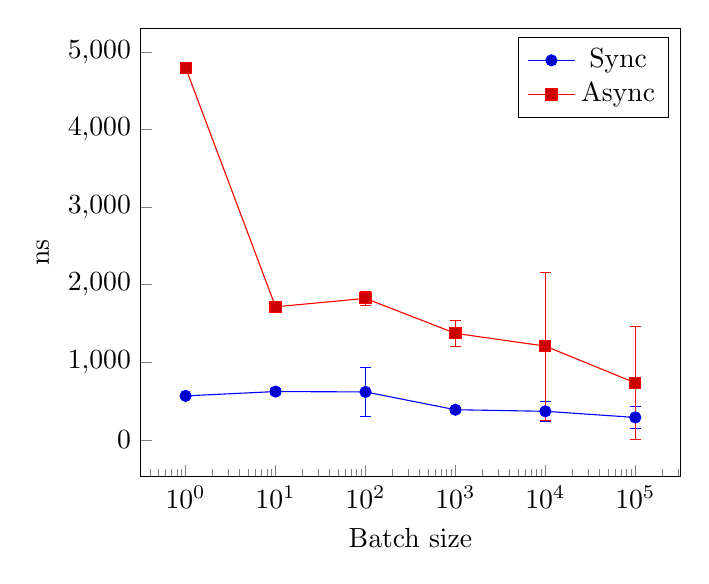
\begin{tikzpicture}
    \begin{axis}[
      xmode=log,
      xlabel=Batch size,
      xtick pos=left,
      ytick pos=left,
      ylabel=ns]

    \addplot+[
      error bars/.cd,
      y dir=both,
      y explicit]
      coordinates {
        (1, 568.40) +- (0.0, 23.55)
        (10, 624.37) +- (0.0, 35.23)
        (100, 619.51) +- (0.0, 312.56)
        (1000, 390.10) +- (0.0, 33.70)
        (10000, 369.93) +- (0.0, 125.09)
        (100000, 290.79) +- (0.0, 141.02)
      };

    \addplot+[
      error bars/.cd,
      y dir=both,
      y explicit]
      coordinates {
        (1, 4795.77) +- (0.0, 27.21)
        (10, 1715.96) +- (0.0, 32.29)
        (100, 1824.03) +- (0.0, 91.67)
        (1000, 1374.05) +- (0.0, 166.80)
        (10000, 1209.43) +- (0.0, 953.92)
        (100000, 735.62) +- (0.0, 724.98)
      };
      
      \legend{Sync, Async}
    \end{axis}
  \end{tikzpicture}
  \caption{Sync in-memory time recorder and Async in-memory time recorder performance comparison}
  \label{fig:timerecorerimplementation:performancecomparison}
\end{figure}

\noindent The batch size roughly correlates with $n$ when the software will measure the algorithm under test. Because there is no real work being done in these microbenchmarks besides calling the time recorder methods, the actual performance of the time recorders could differ when used while measuring the algorithm under test. Nevertheless, the sync time recorder never takes more than 
\SI{1}{\micro\second} which means it should not have a big impact on the observer effect. The async time recorder is a bit slower and performs better with bigger batch sizes.

\noindent The major problem the sync time recorder has is that the data it stores in memory might not fit in the physical space allocated for the JVM process as it stores all the data that it receives in its raw format. The raw data is not needed for the time complexity to be estimated. Instead, the total time spent in each method in a specific call path and how many times each method in a specific call path is called is what is needed. Because everything runs in a single thread, it is not possible to do the necessary calculations to keep the memory usage at a minimum without impacting the observer effect. The async time recorder addresses that problem by doing the calculations in a separate thread and storing the results in a call tree where only the data needed to calculate the time complexity is kept.

\noindent The other disadvantage the sync time recorder has is that when it is stopped, the processing of that data to transform it into a call tree might take too much time. Despite this does not have an impact on the observer effect, it still has an impact on the time needed to estimate the algorithm time complexity. As mentioned before, the async time recorder builds the call tree as the data is received taking advantage of more CPU cores, meaning that when it is stopped it can return it straight away without any additional processing.

\noindent Given these considerations, the sync time recorder should be used when accuracy is essential and there is enough memory in the system to store all the data. The async time recorder should be used when speed is more important than accuracy but should always be avoided on machines that only have a single-core CPU.

\noindent Note that because the implementation is abstracted away using the time recorder API, it is very easy to come up with new and potentially more performant implementations. Some ideas include flushing the data to disk in a separate thread (i.e. async on-disk time recorder), writing to a database or streaming the data to a remote machine. It is also possible to create a hybrid of the two implementations described above, using the sync version for small batches and the async one for big batches. All of these ideas are outside of the scope of this dissertation.

\section{Time complexity analysis SDK}

TODO by 07/08


\section{Algorithm under test}

TODO by 14/08


\section{Time complexity analyser}
\label{sec:implementation:timecomplexityanalyser} 
TODO by 21/08
